%
% File naaclhlt2016.tex
%

\documentclass[11pt,letterpaper]{article}
\usepackage{naaclhlt2016}
\usepackage{times}
\usepackage{latexsym}
\usepackage{graphicx}
\usepackage{url}
\usepackage{xcolor}
\usepackage{amsmath}
\usepackage{amssymb}
\usepackage{multirow}
\usepackage{booktabs}

% nicer URLs
\makeatletter
\def\url@leostyle{%
  \@ifundefined{selectfont}{\def\UrlFont{\sf}}{\def\UrlFont{\scriptsize\sffamily}}}
\makeatother
% Now actually use the newly defined style.
\urlstyle{leo}


\newcommand{\DEVELOPMENT}{1} % 1= show comments, 0=no comments
\usepackage{ifthen}
\ifthenelse{\DEVELOPMENT = 1}{
	\newcommand{\tz}[1]{\textcolor{cyan}{\textbf{TZ:} #1}}		
	\newcommand{\mw}[1]{\textcolor{red}{\textbf{MW:} #1}}		
	\newcommand{\om}[1]{\textcolor{magenta}{\textbf{OM:} #1}}		
}{
	\newcommand{\tz}[1]{}		
	\newcommand{\mw}[1]{}		
	\newcommand{\om}[1]{}		
}
\DeclareMathOperator*{\argmax}{arg\,max}

%\naaclfinalcopy % Uncomment this line for the final submission
\def\naaclpaperid{***} %  Enter the naacl Paper ID here

% To expand the titlebox for more authors, uncomment
% below and set accordingly.
% \addtolength\titlebox{.5in}    


\title{Bundled Gap Filling: A New Paradigm for Cloze Exercises with no Distractors}

% Author information can be set in various styles:
% For several authors from the same institution:
% \author{Author 1 \and ... \and Author n \\
%         Address line \\ ... \\ Address line}
% if the names do not fit well on one line use
%         Author 1 \\ {\bf Author 2} \\ ... \\ {\bf Author n} \\
% For authors from different institutions:
% \author{Author 1 \\ Address line \\  ... \\ Address line
%         \And  ... \And
%         Author n \\ Address line \\ ... \\ Address line}
% To start a seperate ``row'' of authors use \AND, as in
% \author{Author 1 \\ Address line \\  ... \\ Address line
%         \AND
%         Author 2 \\ Address line \\ ... \\ Address line \And
%         Author 3 \\ Address line \\ ... \\ Address line}
% If the title and author information does not fit in the area allocated,
% place \setlength\titlebox{<new height>} right after
% at the top, where <new height> can be something larger than 2.25in
\author{Author 1\\
	    XYZ Company\\
	    111 Anywhere Street\\
	    Mytown, NY 10000, USA\\
	    {\tt author1@xyz.org}
	  \And
	Author 2\\
  	ABC University\\
  	900 Main Street\\
  	Ourcity, PQ, Canada A1A 1T2\\
  {\tt author2@abc.ca}}

\date{}

\begin{document}

\maketitle

\begin{abstract}
Very abstract
\end{abstract}

\section{Introduction}
\begin{itemize}
	\item cloze tasks like (see Figure 1a) are frequently used in language learning. They are hard to automate as there might be more than one valid solution (see example)
	\item Ambiguity of cloze tasks is countered with distractors (at the cost of changing the nature of the task). Problem remains, distractors might still be valid in the given context. Have to be chosen very carefully, hard to do automatically (see REFERENCES).
	\item For a task to be useful, it needs to be of a certain difficulty and valid at the same time. With distractors the trade-off is hard to resolve, when choosing distractors that have little relatedness with the target word, we usually get valid but very easy tasks. All methods from the literature that try to select more difficult distractors face the (so far) unsolved challenge to ensure validity.
	\item we propose to `solve' the problem, by switching to a related paradigm that tests similar knowledge, but where it is easier to control the task difficulty
	\item instead of showing one sentence with a gap and distractors, we propose to show multiple sentences with gaps where the same word is replaced in each sentence EXAMPLE
	\item FIGURE comparing the approaches. a) cloze, b) cloze+distractors, c) context bundles
\end{itemize}

\om{Also, we need to stress that we automatically generate the exercises right from the start. I think that manually generating our proposed exercises is much more difficult than manually generating distractors, so in our case the importance of the NLP automation is even greater.}

\section{Related Work}

\om{It would be nice  to have there some background about ambiguity of cloze tests (when no distractors are used), and on the importance of automatically generating exercises.}
\tz{at(MW): can you add some text about this from your master thesis (or the old paper draft)?}

\paragraph{Validity}
blub
\paragraph{Difficulty}
blub
\vspace{5mm}

\newcite{Zesch2014} use context-sensitive lexical inference rules in order to generate distractors that are semantically similar to the gap target word in some sense, but not in the particular sense induced by the gap-fill context.
While their approach points in a promising direction it fails to model a sufficient large difficulty continuum - especially when targeting a a group with high level of language proficiency. 


\tz{Copied from our 2014 paper. a starting point, but needs to be heavily adapted. Mainly for the purpose of having all the references.}
The process of finding good distractors involves two steps: \emph{Candidate Selection} controls the difficulty of the items, while \emph{Validity Checking} ensures that the item remains solvable, i.e.\ we need to ensure that distractors are not just another correct solutions.

\subsection{Selecting Distractor Candidates}
In some settings, the set of possible distractors is known in advance, e.g.\ the set of English prepositions in preposition exercises \cite{Lee2007} or a confusion set with previously known errors like \{two, too, to\}.
\newcite{sakaguchi-arase-komachi:2013:Short} use data from the Lang-8 platform (i.e.\ a corpus of manually annotated errors) in order to determine the confusion sets.
In all other cases, only the target word is known and the set of distractors needs to be determined.

Randomly selecting distractors is a valid strategy \cite{Mostow2012}, but it is only suitable for the most basic learners.
More advanced learners can easily rule out distractors that do not fit grammatically or are semantically too unrelated.
Thus, more advanced approaches usually ensure that distractors have the same POS tag as the target word.
Additionally, some approaches \cite{Hoshino2007} rely on distractors having a corpus frequency comparable to the target word (based on the assumption that corpus frequency roughly correlates with word difficulty).

In order to make distractors more challenging, one can use thesauri \cite{Sumita2005,Smith2010} or taxonomies \cite{Hoshino2007,Mitkov2009} to select words that are semantically similar to the target word.
\newcite{Pino2009} use distractors that are morphologically, orthographically, or phonetically similar, e.g.\ \emph{bread -- beard}.
Instead of only looking at the target word, some approaches consider the semantic relatedness of distractors with the whole carrier sentence or paragraph \cite{Pino2008,Agarwal2011,Mostow2012}, i.e.\ they pick distractors that are from the same domain as the target word. \mw{local context not really considered}

Generally, selecting more challenging distractors usually means making them more similar to the target word.
As this increases the probability that a distractor might actually be another correct solution, we need a sophisticated approach for checking the validity of a distractor.

\subsection{Judging Distractor Validity}
In order to make gap-fill items more difficult, we have to get close in meaning to the target word, sometimes too close.
Thus, we need a reliable way to judge whether a distractor is valid, i.e.\ that it does \emph{not} fit into the context of the carrier sentence.

In those cases, where we have a limited list of target words and distractors, e.g.\ in preposition exercises \cite{Lee2007}, we can train a supervised classifier.
Given enough training data, this approach yields a very high precision, but it cannot be easily applied to open word classes like nouns or verbs, where the confusion sets are not known in advance.
Additionally, we would need to train a very high number of classifiers. 
In case that we do not have a list of challenging distractors at hand, we might be still able to limit the scope in which a certain target word can appear by looking for collocations involving the target word \cite{Pino2008,Smith2010}.
For example, if the target word is \emph{strong}, we find the collocation \emph{strong tea} and can use \emph{powerful} as a distractor, because \emph{*powerful tea} is not a valid collocation.
While collocations are an important part of language knowledge and should be trained accordingly, collocations need to be strong enough to rule out a sufficient number of invalid distractors.
The approach also limits the set of carrier sentences to those containing a strong collocation.
For example, we would not have been able to use the sentence in Figure~\ref{fig:example} as it contains no usable collocation.

\newcite{Sumita2005} apply a simple web search approach to judge the validity of a distractor.
They check whether the carrier sentence with the target word replaced by the distractor can be found on the web.
If such a sentence is found, the distractor is discarded as invalid.
However, the applicability of the approach is limited, as finding exact matches for sentences is rather unlikely, i.e.\ not finding such a sentence does not necessarily rule out the possibility of an invalid distractor.

To summarize: A reliable method for judging the validity of a distractor in any given context is still to be found.
We propose to use contextualized entailment rules for this purpose and describe the approach in the next section.

\section{Bundled Gap-Fill Exercises}
We propose \textit{Bundles Gap-Fill Exercises} as a new paradigm where instead of choosing suitable distractors for a single sentence in order to reduce ambiguity, we select a set of sentences that together reduce ambiguity.

\om{Again, I suggest we stress that this is not just a different way of addressing ambiguity and controlling difficulty, but the nature of the exercise is different and hopefully/possibly more appealing (generation vs. ranking).}
\om{It may be helpful be to put here a pseudo-code diagram that describes the process of generating the minimal-set bundle in very high level. Then we can explain the steps in more detail.}
The sentence contexts should be chosen in a way that they make all other solutions highly unlikely under a common-sense interpretation.
For example, in the sentence \textit{`They \_\_\_ in the committee for one period'}, where \textit{serve} was the original word, but \textit{work} would be an equally likely solution. \tz{Should be checked by native speaker}
This ambiguity can be resolved by choosing another sentence where \textit{serve}  is also used as the target word, but \textit{work} is less likely, e.g.\ \textit{`Please \_\_\_ the tea'}.
When used together, the only likely solution is \textit{serve}.
We call the smallest set of $k$ sentences that only have a single solution for a shared gap $g$ a \textit{minimal sentence bundle}. \tz{:)}
In order to find such a bundle, we need to know the probability of other possible solutions for a given gap.
For this purpose, we will use substitute vectors.

%Basically, this approach does not change the underlying testing paradigm of reduced redundancy testing \cite{spolsky1969reduced}, as one still needs to infer a solution from context with reduced redundancy (i.e.\ the context has a gap).
%However, the proposed approach offers the advantages of a gap-fill task without distractors (i.e.\ the solution is not provided to the person to test and therefore there is no bias) without having its disadvantage of multiple possible solutions. 

\subsection{Obtaining Substitute Vectors}


For each sentence in our set of candidate sentences, we can compute a substitute vector where all possible gap fillers are scored according to how well they fit the gap.
We will use a language model
\tz{Oren could you write some details about the fastsub language model?}
\tz{theoretical advantages/disadvantages of using other models, e.g.\ paradigmatic substitutes from a second-order DT?}

Exemplary, the output of this process is shown in figure \ref{fig:mostProbableVector}.
\begin{figure*}
	\centering
  		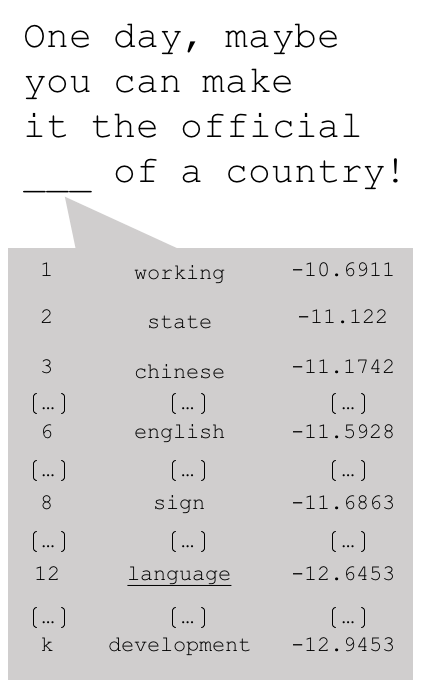
\includegraphics[width=0.3\textwidth]{figures/example_most_probableVector.png}
  		\caption{Example of a weighted vector containing the substitutes associated with the probability they fit into the gap.  \mw{ordering rauslassen? im Beispiel etwas schummeln damit es schöner aussieht und klarer wird?} \tz{Rank würde ich weglassen, genaue Visualisierung muessen wir nochmal diskutieren.}}
  		\label{fig:mostProbableVector}
\end{figure*}

\subsection{Finding a Minimal Set}
Given these substitute vectors, we can start to search for a \textit{minimal sentence bundle} for a target word $t$ from a sentence base $S$.
Since we want to select a \textit{sentence bundle} for $t$, the sentence base is restricted to all sentences $S_t$ that contain $t$.
For finding \textit{minimal sentence bundle} a straightforward approach would be to first form all possible combinations of all sentences $s \in S_t$ and then evaluate them on how ambiguous they are.
This exhaustive search is not useful from a practical point of view as it would result $O(n^k)$ computations.
We therefore propose to utilize a greedy algorithm with complexity $O(n)$.

\paragraph{Seed Sentence}
We select as seed sentence, the sentence $s \in S_t$ where $t$ has the highest weight, as a high weight means that $t$ is very probable in $s$ and therefore that $s$ is a typical context of $t$. 

\paragraph{Next Sentence}
\tz{This needs to be shortened and expressed more clearly}
After having found the seed sentence, we proceed with the greedy algorithm to search for other contexts that resolve as much ambiguity as possible.
In other words, contexts are needed that result in different substitute vectors for $t$.
In order to decide this algorithmically, a measure is needed to express the amount of reduced ambiguity.
While maximizing the reduction of ambiguity, it needs to be ensured that the initial target word is still a valid solution to both tests at the same time.
Otherwise, most ambiguity could be resolved by choosing a context with no relation to the target word.
As a consequence, the fitness-measure needs to model both the likelihood of the target words and the the un-likelihood of all other candidates according to a set of vectors.
Or expressed differently, the set needs to maximize the probability of the target word while simultaneously the probabilities of all other possible substitutes are minimized. 
Basis of such a measure is the ability to compare the resulting probability of different substitutes across a set of sentences.
We accomplish that by averaging the weights of substitutes over the different vectors.
This means, we compute the probability of a single substitute to be the solution to $j$ sentences $S_j$ by the formula:
\begin{equation}
\label{eq:coreMeasure}
	p_{S_j}(x)=\dfrac{\sum\nolimits_{S_i \in S_j}p_{S_i}(x)}{j} 
\end{equation}
Consequently, the fitness-measure of a set of $j$ sentences $S_j$ with a set of dimensions $D$ can be computed by comparing the probability of $t$ and the probability of all other substitutes: 
\begin{equation}
\label{eq:coreMeasure}
	v(S_j)=p_{S_j}(t)-\dfrac{\sum\nolimits_{w_i \in D^*}p_{S_j}(w_{i})}{\vert D^* \vert} 
\end{equation}
	where $w_i \in D^*$ with $w_i \neq t$ are all substitutes in $S_j$ except the target word $t$ and $\vert D^* \vert$ is the cardinality of $D$ without $t$.
Consequently, the approach assumes that the best achievable validity is given for $\argmax_{S_j \in S}(v(S_j)) $. 
This procedure is exemplified in figure \ref{fig:secondStep}. 
\begin{figure*}
	\centering
  		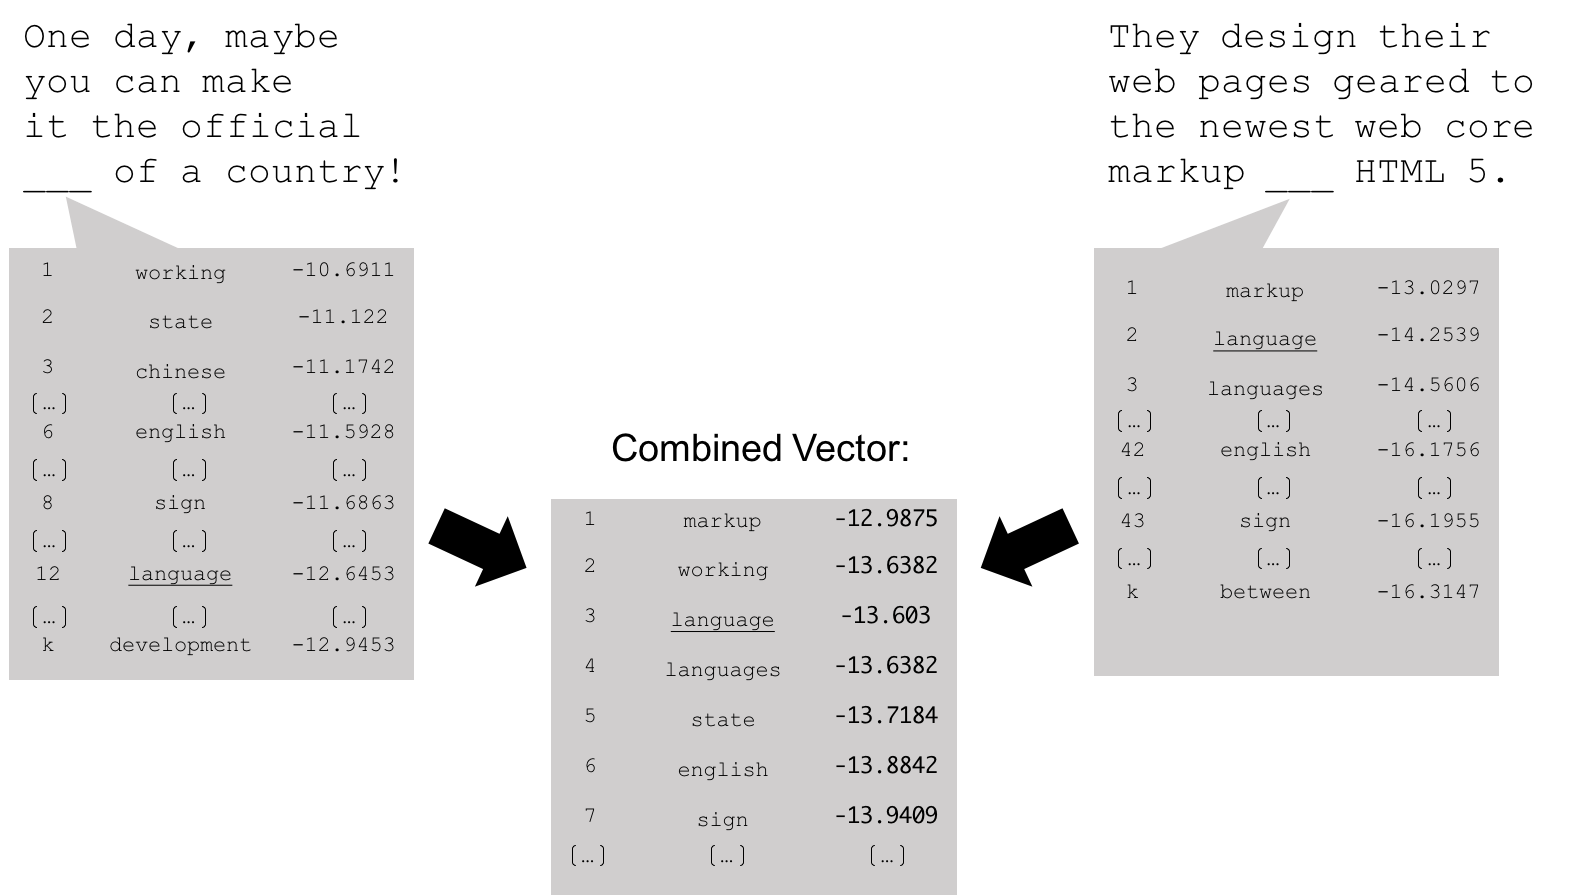
\includegraphics[width=0.7\textwidth]{figures/example_second_context.png}
  		\caption{A second context is chosen by maximizing the proposed fitness-measure. \mw{links im context fehlt 'languages'}}
  		\label{fig:secondStep}
\end{figure*}
	
For reasons of simplicity and performance, we use substitute vectors that are pruned to the $k$ most probable substitutes. 
However, this has the consequence that the vectors may consist of differing dimensions - respectively differing substitutes. 
This is problematic, since when calculating the mean weight of a dimension ($p_{S_j}(x)$) there might be no weight for $x$ for a certain vector. 
The weight of $x$ could have any value between the value of the $(k+1)$\textit{th} element of the vector (whose exclusive, upper bound is the value of the $(k)$\textit{th} element) and the most unlikely element (whose exclusive, lower bound is zero).  
Hence, we use the weight of the $(k)$\textit{th} element for $p_{S_j}(x)$, since this represents the most conservative estimate of the weight of $x$.

\paragraph{Stopping Criterion}
Either choose $k$ sentences or stop at some other criterium
\tz{what would be a good choice? delta between probability of target at first rank and next best candidate?}


\section{Generating Exercises}	
As described in the previous section, an actual instantiation of the presented algorithm is dependent on the three following input resources:
	 \begin{itemize}
  		\item a (large) sentence base
  		\item a language model as the basis for the computation of substitute vectors
  		\item a target word as an anchor for the computation of substitute vectors
	\end{itemize}
In the following, it will be described which resources are used and how additional parameters are tuned for our evaluation scenario that will be presented in section \ref{sec:evaluation}.

\subsection{Language Model}
\om{Generally-speaking, references from year 1999 regarding common practices of using language models would be considered outdated (e.g. the size of the corpora that can be used now is order of magnitudes larger). I suggest looking for more recent references. One reference that you should use is my NAACL 2015 paper. Just say that you're following the configuration that worked well in this previous work.}
\om{I don't think you need to get into the details of how FASTSUB achieves its efficiency. Just say that it is efficient and refer interested readers to the original paper.}
Basis of the presented algorithm are the substitutes produced. 
Therefore, the quality of this substitute production is crucial. Empirical studies on language modeling show that the performance of language models is strongly dependent on the size of the corpus they are trained on \cite{chen1999empirical}. 
Thus, we need a sufficient large corpus to train our model. 
Further,  we want to reflect actual usage of language rather than one that is proofread by professional editors (as in news corpora), as this might result in an bias to a certain style and unnatural usage of language.
In contrast, it should also be avoided that incorrect usage affects the model.  
Hence, we argue that a corpus create from the web meets our requirements best, as it reflects a balance between everyday (and partly faulty) and edited use of language. 
That is why we use the \textit{ukwac} corpus \cite{baroni2009wacky} to train our model. 
In addition, the performance of language models depends on the size of sequences which are modeled but is stagnating for $N>5$ \cite{chen1999empirical}. 
Consequently, we trained a $5$-gram language model on \textit{ukwac} using the tool KenLM \cite{Heafield-estimate}\footnote{http://kheafield.com/code/} which uses the state-of-the-art smoothing technique \textit{modified Kneser Ney} smoothing. 
In order to actually compute the substitutes we used the efficient FASTSUBS algorithm \cite{yuret2012fastsubs}\footnote{https://github.com/denizyuret/fastsubs-googlecode}. 
The FASTSUBS divides the exhaustive search - that would be needed to all sequentially use all unigrams - in a number of substitute queues that are processed in a terminating tree structure.
Therefore, FASTSUBS complexity is sublinear \cite{yuret2012fastsubs} and well suited for our approach. 

\subsection{Sentence Base}
\om{the sentences should rarely be longer than 9 tokens" - the sentences were longer in the examples that you sent me (?). I agree that shorter sentences are better, maybe also for the learner, but I don't think this should be presented as a hard limitation of our model. It could still work reasonably well with longer sentences (and we can say in future work that better language models that take longer contexts could be used in the future)}
The sentence base from which the contexts are chosen should be as similar as possible to the corpus used for training the model so that its decisions are as rarely as possible based on unknown $N$-grams. 
Since a $5$-gram language model can model a context of 4 proceeding/following words at maximum, the sentences should rarely be longer than 9 tokens. 
In addition, the sentence base needs to have a sufficient size it should offer enough distinct contexts for a target word to choose from. 
However, since the size of the sentence bas is a large influencing factor of computational complexity, the size should not exceed a practicable size.
As a result, the GUM corpus \cite{zeldesgum}\footnote{https://github.com/amir-zeldes/gum} seems to meet these requirements, as it is rather small sized (44\,000) and extracted from the web. 
In addition, the  
\mw{The GUM corpus is used as well for extracting the target words}

\subsection{Number of Sentences}
In addition to the used resources, our approach relies on the parameter $j$ for the number of desired contexts.
The instantiation of $j$ might be associated with problems for both setting $j$ too small and too big. If $j$ is too small, ambiguity is not sufficiently reduced to produce a valid task.
If $j$ is too big, the person to be tested needs to process to many alternatives simultaneously what may result in cognitive overload respectively shifts the nature of the task from a language proficiency test to a test of human working memory. 
With respect to distractors, it can be shown that three distracters plus the correct answer is the optimal number to provide \cite{graesser2001question}. 
Therefore, we use $j=4$ in our initial experiments. 

\subsection{Selection of Target Words}
Finally, our approach needs one or several target words as an input that could basically any word that occurs more often than $k$-times in the sentence base. To make the sentence bundle tests comparable with other language proficiency tests, the target words are selected by a systematic process from all unigrams in the GUM corpus. 
It can be shown that higher lengths of the omitted words - expressed their count of letters or syllables - results in an increased difficulty of the gap \cite{abraham1992meaning,brown1989cloze}. 
Hence, we control for frequency of the target words by selecting an equal number the frequency spectrum. 
In order to make the frequency controllable, the spectrum of frequencies was partitioned into frequency ranges. Since the distributions of frequencies (ordered decreasingly) follows a power-law \mw{cite?} , the partition is done using powers of ten. 

The findings of \newcite{kobayashi2002cloze} and \newcite{abraham1992meaning} suggest that the difficulty of a gap is influenced by whether the omitted word is a function word (words with a purely grammatical function) or a content word (words with lexical meaning).
\om{it's not clear how this is related to the rest of the paper. Are you testing both content and function words?}

\section{Evaluation}
\label{sec:evaluation}

The new test format is successful if it creates valid tests


After the conceptual background and the implementation of our new approach have been presented, it is necessary to validate if it meets the assertions. In order to evaluate approach, we compare the resulting sentence bundle tests with the regular gap-fill tests with distractors \mw{oder auch ohne?}. Therefore, we postulate and test the following hypotheses:
\begin{itemize}
  \item Contextualized sentence bundles are suitable to test language proficiency. I.e. the performance in the contextualized sentence bundles is positively correlated with the reported language proficiency. \mw{wir könnten auch Gruppenvergleiche machen mit CRF levels}
  \item Contextualized sentence bundles are better suited than gap-fill tasks with distractors to test language proficiency. I.e. contextualized sentence bundles show a stringer correlation than gap-fill tasks. 
  \item \mw{wollen wir das jetzt noch mit dem einstellen der Schwierigkeit machen?}
\end{itemize}

%\subsection{Test Battery}
%At first we need a reference score of the participants language proficiency.
%Since an objective assessment takes a lot of time and often comes with disputed validity, this work focusses on self-assessment.
%However, self-assessment in second language testing has been found to have different degrees of validity \cite{ross1998self}. 
%It is particularly poor if the participants are asked for a self-assessment after a language test. 
%To prevent this priming effect, which could arise from perceived success or failure in the test, we ask for a self assessment before testing the contextualized sentence bundles and gap-fill tasks.
%Consequently, in accordance with \newcite{leblanc1985self} self-estimated English skills are surveyed for reading, listening and writing with a five staged Likert-scale. 
%Because the English capabilities of a second language learner depends on her personal education and experience, the self-assessment was supplemented by questions about her learning career. 
%Participants are asked how long they learned English in schools, lived or worked in an English-speaking community and for supplementary taken learning opportunities like university courses. 
%In addition to their English career, participants should list all other learned second Languages in the order they were acquired. 
%Finally participants are asked if they have absolved a standardized language test (like TOEFL, IELTS) and |if present| for their gained score.

\subsection{Results}

\section{Discussion}

\subsection{Reintroducing Distractors}
Actually, our model allows to generate distractors (top entries in the joint substitute vector).

\subsection{Conclusions \& Future Work}

In this paper, we have focussed on the validity of the generated exercises.
We see two main lines of future work:
First, we want to better control difficulty ...
Second, we want to determine what kind of knowledge the test is actually measuring.
It might be that this tests measures something completely different than cloze tests.
\tz{This is more in the realm of educational research. We could also just say this is still a cloze test :)}

%\section*{Acknowledgments}
%This work was supported by the Deutsche Forschungsgemeinschaft (DFG) under grant No. GRK 2167, Research Training Group ``User-Centred Social Media''.
 

\bibliography{bea2016.bib}
\bibliographystyle{naaclhlt2016}


\end{document}
